\section{Motivação}
\label{motivacao}

O estudo de linguagens menores que sejam capazes de expressar regras de maneira mais clara não é novidade na área da engenharia de sistemas, \citeonline{bentley} já demonstrava em sua pesquisa diferentes abordagens de construção de pequenas linguagens para facilitar a escrita de programas gráficos e interface gráfica.


\citeonline{wexelblat}, apresenta o termo "linguagem de propósito especial", quando se refere à \gls{JOVIAL}, linguagem de alto nível destinada principalmente para auxiliar na programação de grandes sistemas complexos em tempo real. 

Um exemplo de aplicação dessas linguagens pode ser visto na Figura \ref{fig:piclanguage} em que o compilador transforma comandos simples no formato textual em formato de digrama (Figura \ref{fig:piclanguageresultado}), abstraindo detalhes específicos das linguagens tradicionais de programação da época.

\begin{figure}[ht!]
\centering

\caption{\textmd{Comandos na PIC Language}}
\label{fig:piclanguage}
\fcolorbox{gray}{white}{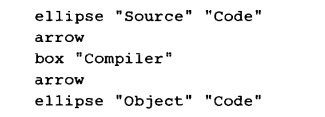
\includegraphics[width=0.67\textwidth]{images/piclanguage}}

\par\medskip\textbf{Fonte:} \citeonline{bentley}. \par\medskip
\end{figure}

\begin{figure}[ht!]
\centering

\caption{\textmd{Diagrama resultado após compilação}}
\label{fig:piclanguageresultado}
\fcolorbox{gray}{white}{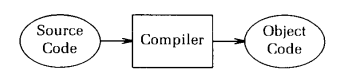
\includegraphics[width=0.67\textwidth]{images/piclanguageresultado}}

\par\medskip\textbf{Fonte:} \citeonline{bentley}. \par\medskip
\end{figure}



Na engenharia de software atual, as Linguagens de Domínio Específico ou \gls{DSL} estão se tornando cada vez mais importantes e as novas ferramentas de criação dessas linguagens são ainda melhores, pois requerem esforço de desenvolvimento relativamente simples \cite{dslengineering}.


A equipe de desenvolvedores do \gls{IFSC} possui uma alta demanda de desenvolvimento de sistemas e serviços internos, atualmente são mantidos mais de 10 sistemas em uso, alguns deles são subdivididos em vários módulos \cite{catalogoifsc}. A \gls{DTIC} centraliza e mantém a maioria dos sistemas e serviços de TI, contando com apenas 12 analistas da tecnologia da informação, além de ter que prestar suporte para todas as 23 unidades da instituição. 

Como agravante, o sistema de ingresso foco deste trabalho, foi criado em meados dos anos 2000 por bolsistas que já não estão mais na instituição, e atualmente apenas 2 desenvolvedores ficaram responsáveis pelas demandas de desenvolvimento e suporte. Por se tratar de um sistema legado criado em linguagem PHP sem qualquer preocupação com documentação ou qualidade de código, o custo de alterações mais complexas como no caso de regras de classificação acaba por atrasar a adequação aos novos requisitos de lei. 

Até o momento, a equipe participou do desenvolvimento de 3 (três) versões do algoritmo de classificação, além de prestar manutenção corretiva em função de entendimentos equivocados nas regras implementadas.  Os algoritmos envolvidos, assim como o seu histórico de versionamento serão detalhados no Capítulo \ref{chap:historicoversoes}.

O Capítulo \ref{chap:proposta} apresenta a proposta de uma Linguagem de Domínio Específico para especificação de regras de classificação de candidatos, na qual usuários especialistas do sistema de ingresso possam estabelecer as categorias de cotas, com objetivo de reduzir o esforço do desenvolvimento e de entendimento das regras de negócio, por parte dos desenvolvedores do sistema, sempre que forem alterados os documentos de lei envolvidos.

Nas seções \ref{problema}, \ref{objetivos}  e \ref{metodologia}, serão apresentados, respectivamente, o problema de pesquisa, as hipóteses, os objetivos e por fim a metodologia de pesquisa utilizada.
